\section{实验}
\label{exp}

\subsection{设置}
\label{exp-setup}

\paragraph{模型与提示。} 我们在相同的任务与环境设置下评估多种智能体。每个智能体只能获得任务描述、应用入口 URL 和登录凭据；参考解法、验证器、数据库模式与后端 API 均不提供。提示中只包含一般规则：通过浏览器操作，依据观察到的页面内容行动，维持跨应用上下文，并在完成后输出 \texttt{done}。对于多模态任务，图像和 PDF 仅以文件路径提供，不附带预解析标注。

\paragraph{基于浏览器的执行。} 所有智能体均使用 \textsc{browser-use}~\cite{browseruse} 运行。该浏览器自动化框架支持 AI 智能体通过浏览器动作进行网页交互。智能体观察渲染后的 DOM 和视口截图，再从受限动作中进行选择，包括导航、点击、输入、滚动、抽取、文件读写以及 \texttt{done}。JavaScript 执行以及对数据库、后端 API、主机文件或验证器的特权访问均被禁用。每项任务开始前，Docker 环境都会重置到预定初始状态；所有运行采用相同的超时时间、失败次数上限、步数预算和日志设置。系统记录包含动作、观察、中间工具输出及最终应用状态在内的完整执行轨迹，用于后续分析。

\paragraph{指标。} 每项任务都针对最终应用状态设置带权检查点。我们报告\emph{完全解决分数}与\emph{检查点分数}：前者仅在所有检查点均通过时取 $1$，后者是已通过检查点的权重归一化比例。结果按总体、领域、模态和应用分别报告。这两项指标共同区分长程工作流的严格端到端完成与部分进展。

\begin{table*}[t]
\centering
\small
\caption{\textbf{\datasetname 上的主要结果。}我们报告平均执行步数、各领域检查点分数、各模态总体分数、完全解决分数及总体检查点分数。$^\dagger$ 表示模型仅在纯文本领域上评估，其完全解决分数也只根据纯文本任务计算。}
\label{tab:main_results}
\renewcommand{\arraystretch}{1.12}
\resizebox{\textwidth}{!}{
\begin{tabular}{l c ccccc ccc c c}
\toprule
\multirow{2}{*}{\textbf{模型}} & \multirow{2}{*}{\textbf{平均步数}}
& \multicolumn{5}{c}{\textbf{纯文本}} & \multicolumn{3}{c}{\textbf{多模态}}
& \multirow{2}{*}{\textbf{完全解决}} & \multirow{2}{*}{\textbf{总体}} \\
\cmidrule(lr){3-7}\cmidrule(lr){8-10}
& & \textbf{Business.} & \textbf{Healthcare.} & \textbf{Software.} & \textbf{Teamwork.} & \textbf{总体}
& \textbf{Agriculture.} & \textbf{Media.} & \textbf{总体} & & \\
\midrule
Claude Opus 4.7~\cite{claudeopus47} & 175 & 31.8 & 29.7 & \textbf{52.9} & 47.7 & \textbf{42.8} & 46.3 & 46.3 & 46.3 & \textbf{3.8} & \textbf{43.9} \\
GPT-5.5 High~\cite{gpt55} & 200 & \textbf{36.4} & \textbf{30.9} & 45.8 & 54.6 & 42.1 & 51.7 & 45.2 & 47.6 & 1.9 & 43.8 \\
Claude Opus 4.6~\cite{claudeopus46} & 257 & 33.2 & 27.2 & 41.9 & \textbf{65.2} & 40.7 & 42.0 & \textbf{52.8} & \textbf{48.7} & 1.9 & 43.2 \\
GPT-5.4 High~\cite{gpt54} & 252 & 20.6 & 26.8 & 35.5 & 50.4 & 33.0 & \textbf{53.4} & 41.7 & 46.1 & \textbf{3.8} & 37.0 \\
Kimi K2.6~\cite{kimik26} & 269 & 30.0 & 26.2 & 25.5 & 47.2 & 30.1 & 50.1 & 39.5 & 43.5 & 0.9 & 34.1 \\
Qwen 3.6 Plus~\cite{qwen36plus} & 249 & 15.3 & 18.9 & 20.7 & 44.6 & 23.1 & 52.6 & 41.3 & 45.5 & 1.9 & 29.9 \\
Kimi K2.5~\cite{kimik25} & 270 & 13.2 & 20.2 & 20.8 & 48.4 & 23.6 & 51.3 & 28.5 & 37.0 & 0.0 & 27.7 \\
Gemini 3.1 Pro~\cite{gemini31pro} & 140 & 11.2 & 20.0 & 14.7 & 48.2 & 20.6 & 38.5 & 44.7 & 42.4 & 0.0 & 27.1 \\
Doubao Seed 2.0 Pro~\cite{seed20} & 216 & 10.8 & 13.6 & 22.1 & 33.2 & 19.8 & 46.4 & 42.9 & 44.2 & 1.9 & 27.1 \\
Gemini 3.5 Flash High~\cite{gemini35flash} & 324 & 22.7 & 14.5 & 17.6 & 15.7 & 17.6 & 35.9 & 36.9 & 36.5 & 0.9 & 23.3 \\
Claude Sonnet 4.6~\cite{claudesonnet46} & 155 & 20.5 & 9.5 & 23.9 & 15.2 & 18.7 & 34.1 & 33.8 & 33.9 & 0.9 & 23.3 \\
DeepSeek V4 Pro$^\dagger$~\cite{deepseekv4pro} & 236 & 13.6 & 17.1 & 20.7 & 39.4 & 21.5 & \textemdash & \textemdash & \textemdash & 1.4 & \textemdash \\
GLM-5.1$^\dagger$~\cite{glm51} & 166 & 10.9 & 24.0 & 8.7 & 39.0 & 17.4 & \textemdash & \textemdash & \textemdash & 0.0 & \textemdash \\
MiniMax M2.7$^\dagger$~\cite{minimaxm27} & 256 & 6.9 & 17.7 & 13.6 & 29.9 & 15.8 & \textemdash & \textemdash & \textemdash & 0.0 & \textemdash \\
\bottomrule
\end{tabular}}
\end{table*}

\begin{figure*}[t]
  \centering
  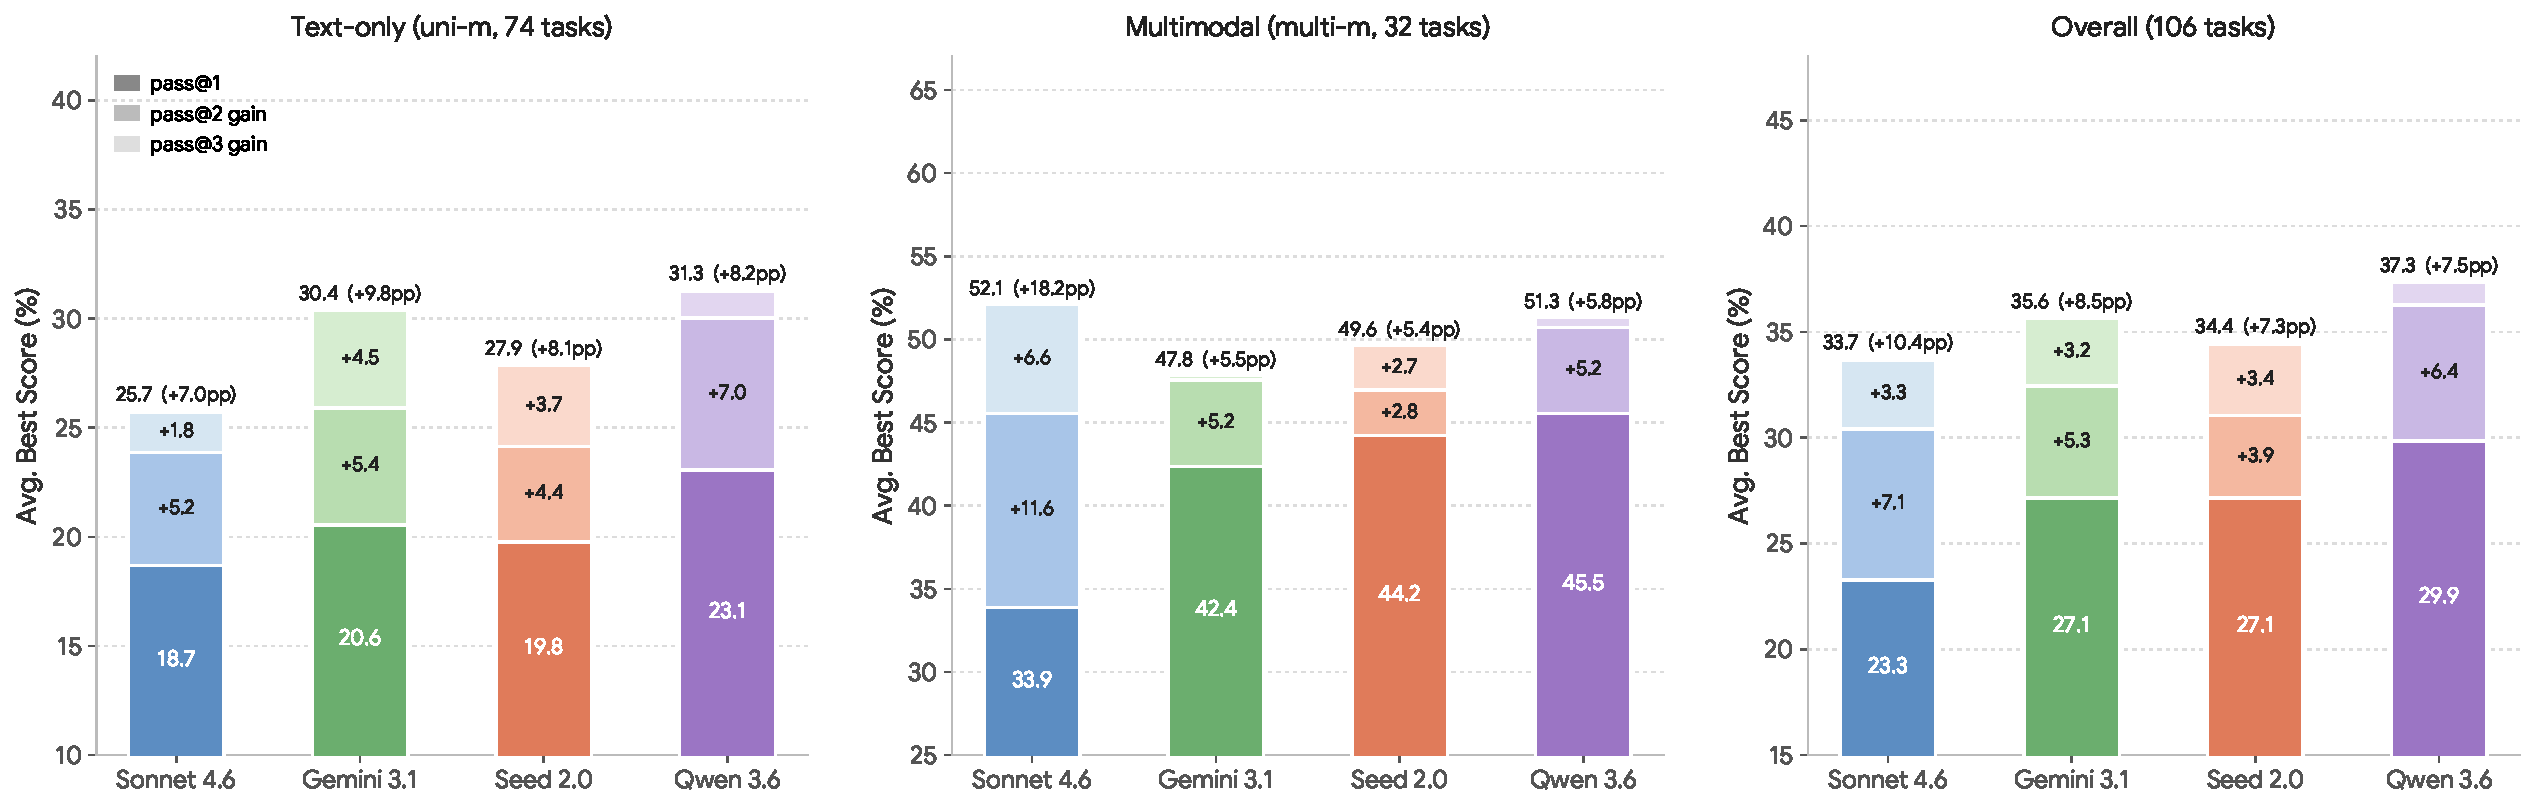
\includegraphics[width=0.8\textwidth]{fig/panel_passk_bar.pdf}
  \caption{四个模型在 \datasetname 的纯文本、多模态和总体三个评测划分上的 Pass@$k$ 平均最佳分数（$k=1,2,3$）。每根柱由三段组成：深色底段表示 pass@1，中间色段表示从 pass@1 到 pass@2 的增益，最浅色段表示进一步到 pass@3 的增益。}
  \label{fig:passk}
\end{figure*}

\subsection{结果}
\label{exp-res}

\paragraph{主要结果。} 表~\ref{tab:main_results} 表明，\datasetname 对当前 CUA 极具挑战。即使最强的 Claude Opus 4.7，总体检查点分数也只有 43.9\%；排名前三的模型（Opus 4.7、GPT-5.5 High 和 Opus 4.6）集中在 43--44\% 区间，其余所有模型均低于 40\%。更值得注意的是，完全解决分数极低：最佳完全解决率仅为 3.8\%，说明智能体往往能完成部分中间检查点，却很少能够端到端完成整个长程工作流。不同领域之间的性能也有差异：Teamwork. 通常比 Business. 与 Healthcare. 更容易，后两个领域要求智能体处理更多结构化记录、数值约束和领域专门流程。总体而言，主要瓶颈在于可靠的长程执行，包括在真实 SaaS 环境中跟踪跨应用上下文、管理状态以及从错误中恢复。

\paragraph{Pass@$k$ 结果。} 图~\ref{fig:passk} 显示，允许多次尝试能够稳定提升性能，但仍不足以弥合差距。在四个代表性模型上，pass@3 相比 pass@1 的总体增幅约为 8 个百分点，表明单次运行层面的方差是 \datasetname 中不可忽视的因素。与此同时，不同模型的收益差异很大：一些智能体能从重复尝试中显著获益，另一些智能体则更稳定但性能较低。这说明许多失败并非完全源于缺乏任务知识，也来自执行不稳定、过早终止或无法从局部错误中恢复。因此，只报告单次 pass@1 分数会掩盖一项重要区别：模型究竟能够稳定完成任务，还是只偶尔找到成功轨迹。这些结果说明，\datasetname 同时衡量单次运行能力与长程执行的一致性。

\begin{figure*}[t]
  \centering
  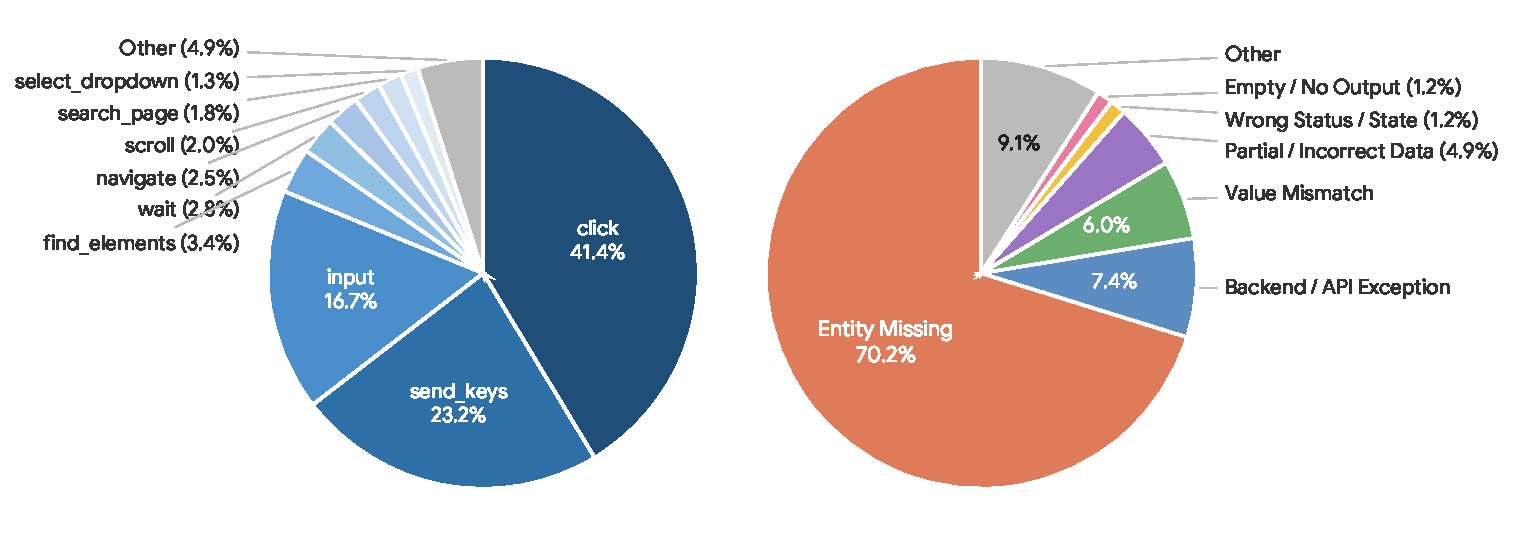
\includegraphics[width=0.82\textwidth]{fig/panel_action_verify_pie.pdf}
  \caption{\textbf{左：}Claude Opus 4.6 在完整基准上输出的底层动作分布；\textbf{右：}按失效模式划分的未通过验证检查。两幅图共同把执行行为与主要失败类型联系起来。}
  \label{fig:pie}
\end{figure*}

\begin{figure*}[t]
  \centering
  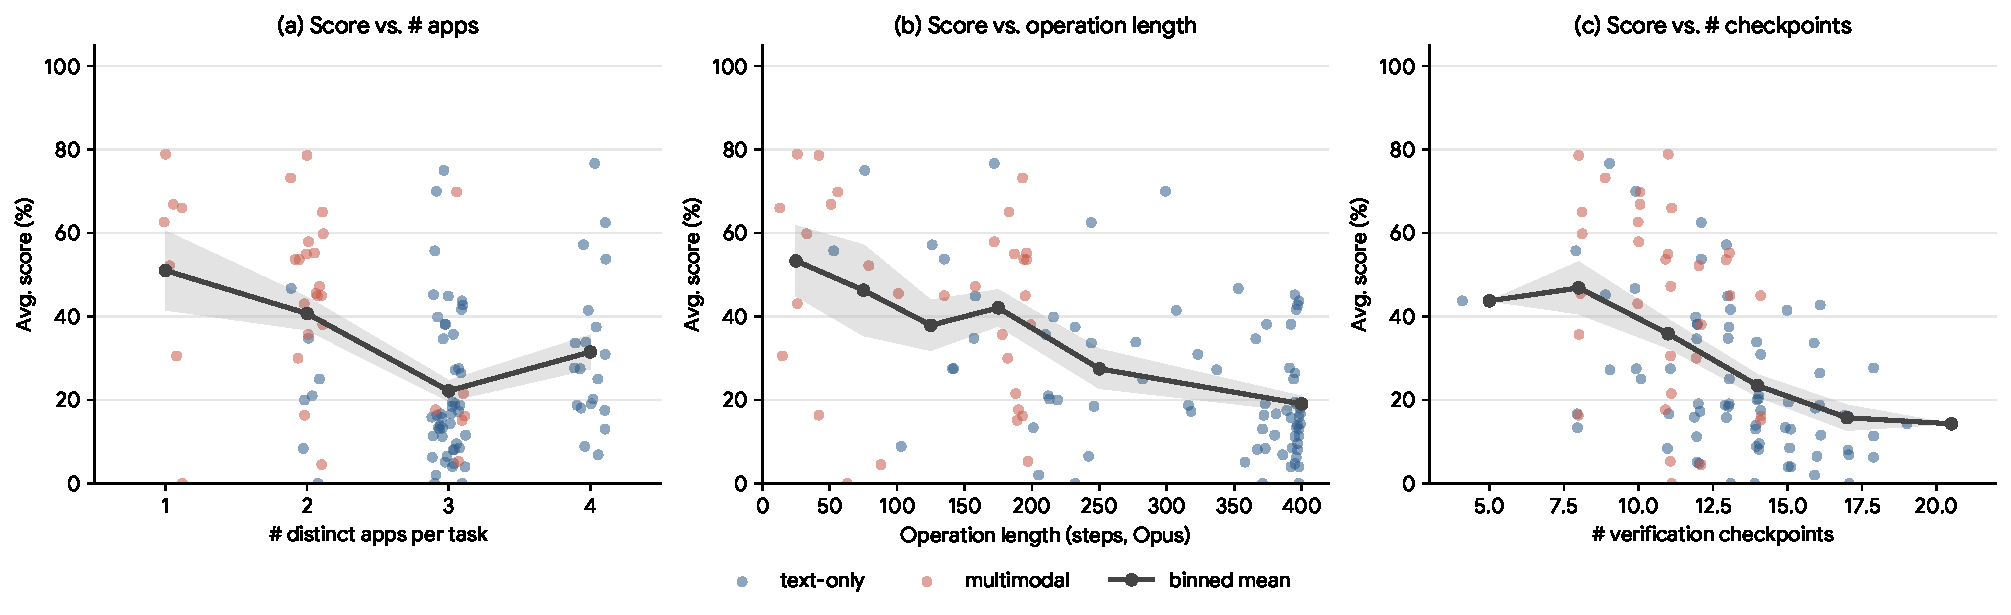
\includegraphics[width=0.86\textwidth]{fig/appx_complexity_combined.pdf}
  \caption{任务分数与三项结构复杂度指标之间的关系：\textbf{左}为任务涉及的不同 SaaS 应用数，\textbf{中}为操作长度（由 Opus 4.6 测得），\textbf{右}为验证检查点数量。每个点代表一项任务；黑线为分箱均值，阴影带表示 $\pm 1$ 个均值标准误（SEM）。}
  \label{fig:appx-complexity}
\end{figure*}

\subsection{分析}
\label{exp-anal}

\paragraph{动作与验证失败分布。} 图~\ref{fig:pie} 给出了智能体动作以及未通过验证检查的分布。左图中，\texttt{click}、\texttt{send\_keys} 和 \texttt{input} 构成了绝大多数已执行动作；下拉选择、页面搜索、滚动和导航等其他操作出现得少得多。智能体如此集中地使用基础交互原语，说明其轨迹的大部分耗费在底层表单填写与导航，而非结构化搜索或系统性页面探索等更高层操作。右图中，失败检查点以\emph{实体缺失（Entity Missing）}为主，即预期记录、文件、工单或其他目标产物根本没有创建。相比之下，取值不符、状态错误或数据部分不正确等失败较少。实体缺失远多于取值层错误，说明首要瓶颈是任务级规划与导航：智能体常常完全没有到达或尝试所需操作，而不是在已经正确识别的步骤上执行不够精确。

\begin{figure*}[t]
  \centering
  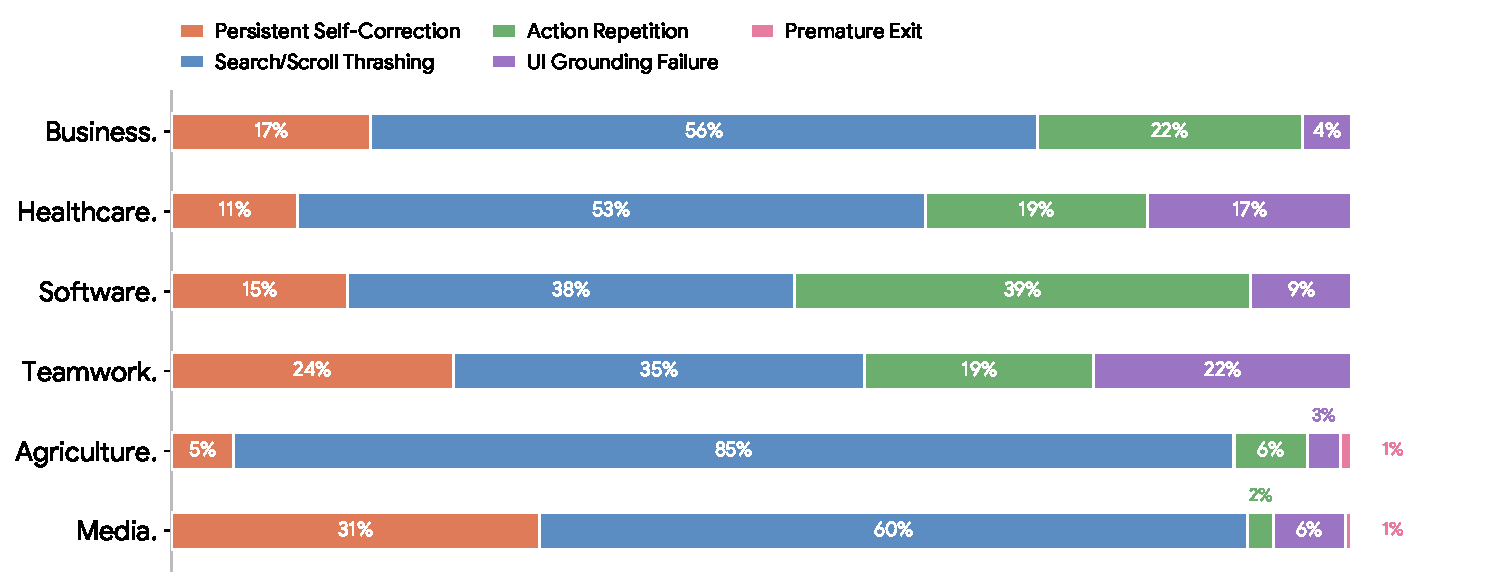
\includegraphics[width=0.82\textwidth]{fig/panel_error_dist.pdf}
  \caption{在 Opus 4.6 轨迹中观察到的智能体行为错误按领域划分后的构成。}
  \label{fig:error}
\end{figure*}

\paragraph{分领域错误分析。} 如图~\ref{fig:error} 所示，失败模式具有显著的领域依赖性，而非均匀分布。在 Agriculture. 与 Media. 这类目录密集型领域，搜索和滚动失败占主导，智能体难以在很长的产品或资产列表中定位目标项。Software. 更常触发在被阻塞或无效控件上的重复动作，这反映了看板、代码编辑器和多面板布局等复杂交互元素的普遍存在。Healthcare. 与 Teamwork. 则暴露出复杂画布和类文档界面中的 UI 定位问题；包含领域术语的密集表单导致字段误识别频发。这种异质性说明，\datasetname 并不能归结为单一 UI 病灶；要取得进展，必须并行改善搜索、定位、重新规划和自我纠错等多项能力。

\paragraph{分数与任务复杂度。} 图~\ref{fig:appx-complexity} 证实，\datasetname 上的分数差距来自任务复杂度，而非随机波动。平均分从最简单任务上的约 $53\%$ 降至最长轨迹任务上的不足 $20\%$；当检查点数量从 $\le 6$ 增加到 $\ge 18$ 时，平均分也从 $65\%$ 降到 $27\%$。跨应用维度（左图）在最多三个应用的范围内呈现同样的单调趋势。值得注意的是，\datasetname 中三个复杂度维度彼此正相关：涉及更多应用的任务往往也拥有更长轨迹与更多检查点。因此，任一维度处于高端的任务，通常在另外两个维度上也同样困难。三幅图共同表明，低分集中在同时具有跨应用、长程和细粒度验证特征的任务上，而这正是 \datasetname 有意施加压力的区域。

\begin{figure*}[t]
\centering
\begin{minipage}[t]{0.48\textwidth}
  \centering
  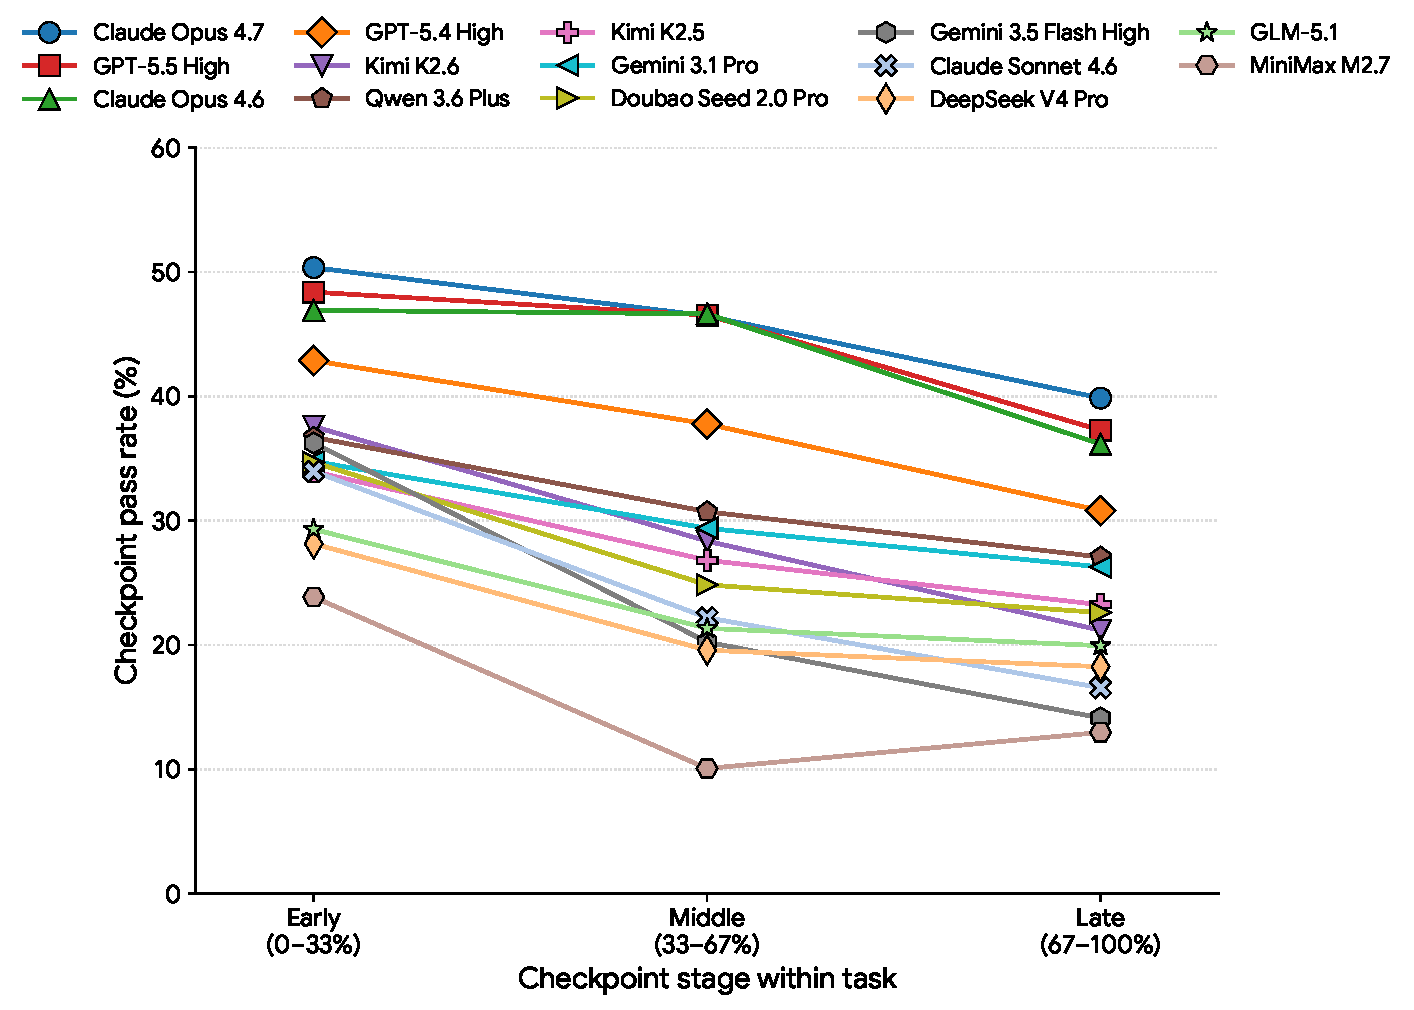
\includegraphics[width=\linewidth]{fig/checkpoint_decay.pdf}
  \caption{按检查点在任务中的位置分层后，各层验证检查点的平均通过率。}
  \label{fig:long_horizon}
\end{minipage}\hfill
\begin{minipage}[t]{0.48\textwidth}
  \centering
  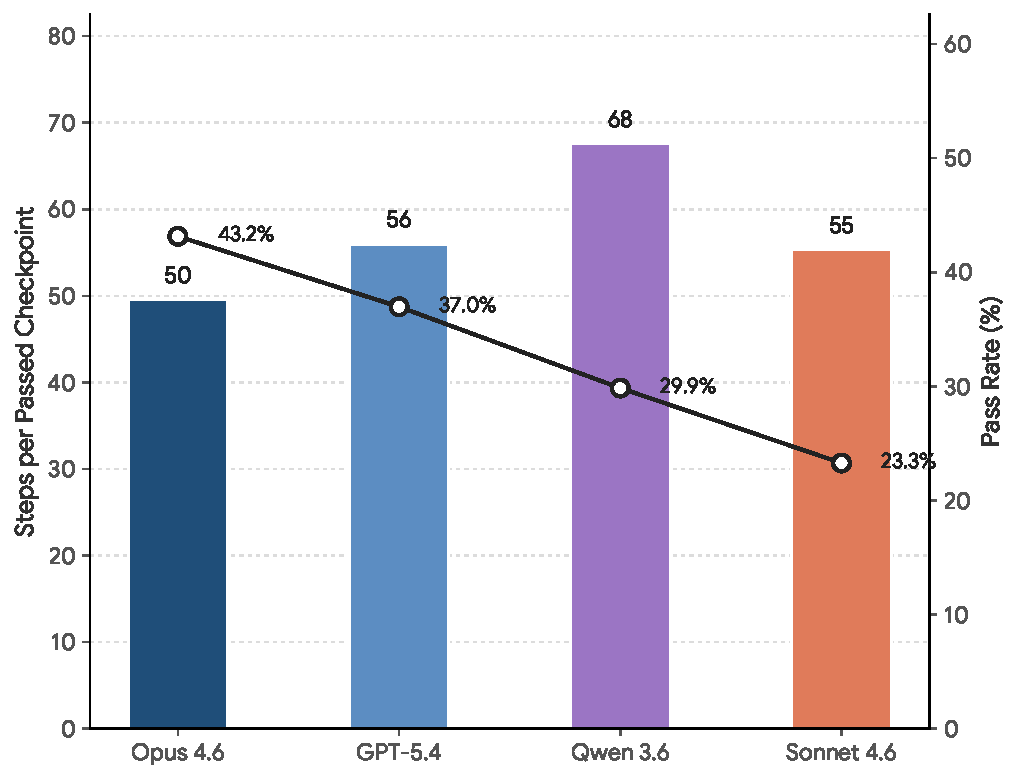
\includegraphics[width=\linewidth]{fig/panel_efficiency.pdf}
  \caption{四个代表性模型每通过一个检查点所需的步数及总体通过率。}
  \label{fig:effic}
\end{minipage}
\end{figure*}

\paragraph{长程检查点衰减。} 图~\ref{fig:long_horizon} 把检查点划分为任务早期、中期与后期，进一步证实了长程瓶颈。所有受评模型都从早期到后期呈现单调下降，说明随着工作流逐步展开，智能体的可靠性不断降低。这种衰减模式在不同能力层级的模型中都一致存在：较强模型在每个阶段都有更高的绝对通过率，但从早期到后期的相对降幅相近。这表明，衰减反映的是当前智能体架构的结构性局限，而非某个模型特有的弱点。该发现也有助于解释表~\ref{tab:main_results} 中检查点分数与完全解决分数之间的巨大差距：汇总检查点分数可能夸大实际任务完成能力，因为智能体或许能完成早期子目标，却无法在工作流后段维持上下文、传递中间结果或完成最终状态更新。

\paragraph{动作效率。} 我们用每个已通过检查点所需步数，衡量模型把轨迹预算转化为任务进展的效率（图~\ref{fig:effic}）。Opus 4.6 的效率最佳，即以最低的每检查点步数成本实现最高通过率；Qwen 3.6 虽然步数很多，却只换来不成比例的少量检查点通过。Sonnet 4.6 的短轨迹反映的是过早放弃，而非真正高效，因为其每检查点成本仍与更强模型相当。这一模式也体现在主要结果中：Gemini 3.5 Flash High 平均消耗最多步数（324），总体分数却接近末尾（23.3\%）；Opus 4.7 使用不到其一半的步数（175），反而取得最高分（43.9\%）。这些结果说明，原始轨迹长度并不能很好地代理能力；较强智能体的区别不在于动作数量，而在于有多少动作真正转化为有意义的任务进展。
